\documentclass{article}
\usepackage{graphicx}
\usepackage{algorithm}
\usepackage{algorithmic}
\usepackage{xcolor}
\usepackage{amssymb}
\usepackage{amsmath}

\newcommand\todo[1]{\textcolor{red}{#1}}
%\newcommand\todo[1]{}

\begin{document}

\title{Template Construction Grammar 1.0}
\author{Victor Barr\`es}

\maketitle

\begin{abstract}
ABTRACT HERE.

\end{abstract}

\section{Introduction}
INTRODUCTION HERE.

\section{Schema Theory}

\paragraph{}
\todo{I MIGHT WANT TO PLACE SOMETHING ABOUT SCHEMA THEORY AT THE BEGINNING!}

\paragraph{}
Here I say a few words about schema theory and how it aims at capture the nature of cognitive processes.
Say that based on schema theory, all the representational formats presented above can be operationalized.
Dynamic operations on symbolic representations: C2 process.
Distinction between \emph{schema} and \emph{schema instances}.
Long term memory structured as a \emph{schema network}.
Schema can be instantiated as schema instances in a working memory. There it can cooperate with other instances to generate \emph{schema assemblages}. Those in turn can compete. etc...
Talk about how this allow for the flexible and dynamic coordination of operations.

The focus of TCG 1.0 is on language schemas

\subsection{Schema}
Define a Schema

\section{Meaning: From visual scenes to semantic representations}
\todo{Here I only have preliminary notes.}
Meaning representation differentiates between high-level visuo-spatial representations and, following conceptualization operation, the semantic representations that can be expressed - transduced-, using grammatical tools, as phonological strings.

Vision-language interface.

\begin{figure}[!htbp]
	\centering
	\includegraphics[width=4.0in]{Figures/Knoeferle&Crocker(04)_Jackendoff97.png}
	\caption{Jackendovian architecture of the language system. Used in Knoeferle and Crocker 04 in relation to the CIA model of situated language processing.}
	\label{jackendoff_arch}
\end{figure}

\subsection{Visual scenes: the structuring role of visual attention}
\todo{Here I only have preliminary notes.}
Going beyond the scope of VISION which focuses on region tagging.
"Regard" through the active process of overt and covert attentional actions (the most obvious ones being saccadic eye movements), on the basis of a current goal (or nexus of goals), generates structured representations of sub-scenes which encompass the information relevant to the current task.

\begin{figure}[H]
	\centering
	\includegraphics[width=4.0in]{Figures/cholitas.jpg}
	\caption{A complex visual scene}
	\label{visual_scene_example}
\end{figure}

Anchored and Minimal subscene.
High level vision gives more than just "tags". The system will assume that such a rich representation is incrementally built through visual attentional processes that are under the control of both bottom-up and top-down factors. Crucially, among the top-down factor will not only figure the overall task, but also requests triggered by the current state of the language system for information.
Multiple loops: The visual attention system is therefore(loosely) coupled with the language system.

Show an example of a scene and the associated sub-scenes.


\begin{figure}[H]
	\centering
	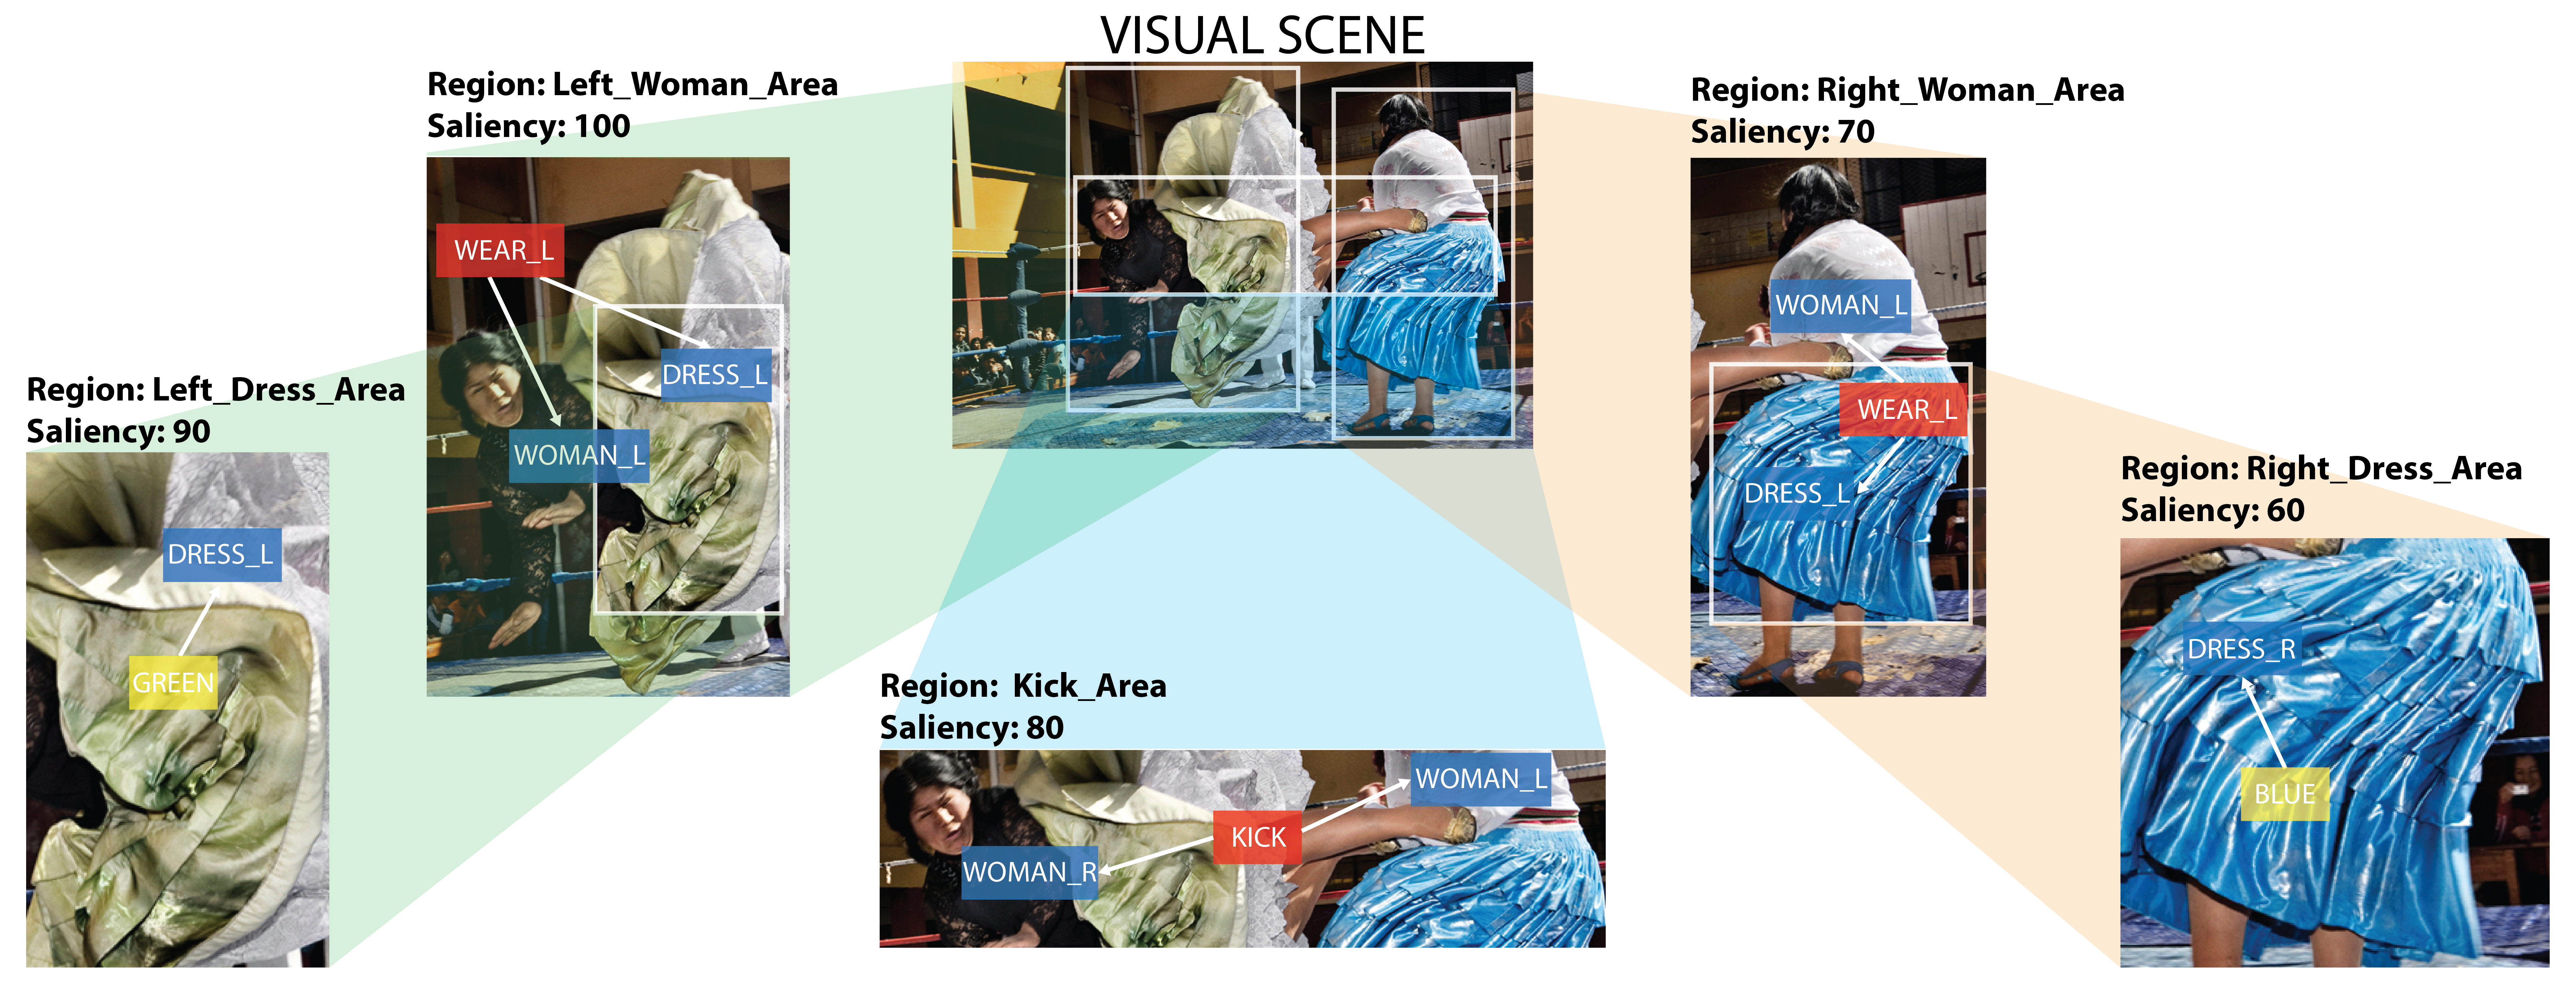
\includegraphics[width=5.0in]{Figures/perceptual_schemas.png}
	\caption{Visual attention and perceptual schemas}
	\label{fig:perceptual_schemas}
\end{figure}

As visual attention is directed to a given region, it is assumed that the perceptual schemas predifined for this sub-part of the visual scene will be instantiated in visual WM.

\todo{Perceptual schemas! Present their formalism.}

\paragraph{Perceptual schemas}
A perceptual schemas can be of two possible type: object or relation. An \emph{object perceptual schema} is defined simply as $(concept, region)$ associating a concept to a spatial region of the visual field. An \emph{relation perceptual schema} is defined as $(relation, (OPS_1, OPS2), region)$ with $OPS_1$ and $OPS_2$ both object perceptual schemas. The relation perceptual schema establishes a relation between two object schemas and is linked to a given spatial region of the visual field.
A given set of perceptual schemas defines a directed graph that capture the perceptual meaning derived from a subpart of the visual scene. 

\paragraph{Percept}
A percept is defined as $(PS, concept)$ associating (mapping) a perceptual schema to a concept. This offer a placeholder model of conceptualization. In its current version, it is redundant with the presence of the concept information as a feature of a perceptual schema (see below for improved version).

\paragraph{Region}
A region is defined $(area, saliency, uncertainty, (PS_i))$ where: $area$ define the location and size of the spatial area of the visual field that corresponds to the region, $saliency \in \mathbb{R}$ defines the bottom-up perceptual saliency of the region, $uncertainty \in \mathbb{N}$ simply serve as a proxy to indicate how hard the visuo-attentional processing of the region is assumed to be, $(PS_i)$ is the list of percepts that will be activated once the region is fixated.

\paragraph{Scene}
A visual scene, that will serve as input to the system is defined as
$$(resolution, width, height, (PS_i), (Region_i))$$ where
resolution, width and height give the basic information about the scene image, $(PS_i)$ is the list of all perceptual schemas associated with the scene, $(Region_i)$ is the list of all the regions defined in the scene. 

\paragraph{Input to model}
The model takes as input a set of regions, each defining: (1) its saliency, (2) the spatial regions it covers, (3) the associated uncertainty, (4) the set of perceptual schemas (object and relations) that compose the perceptual meaning of this region.
These regions are defined in a scene.json input file. \todo{not json yet...}

\paragraph{Attention and visual working memory}
Given the bottom-up saliencies of the different regions but also important top-down factors (see below), the attentional system orients the visual attention in space to one of the scene's region which becomes the focus of attention. The complex perceptual operations required to yield a high-level representation of the region are not modeled (cf. VISION), and the resulting network of perceptual schemas associated with the region is assumed to correspond to the active state of the visual WM. The content of the visual WM is then conceptualized into a semantic representation stored in the semantic WM. Although the process of conceptualization is only hinted at in the model, it represents a key cognitive capacity by which a high level perceptual representation of a scene is abstracted and construed into a semantic structure which is defined purely in terms of linguistic meanings. Such representation is in a form that can then be interpreted by linguistic schemas to generate an utterance.

\begin{figure}[H]
	\centering
	\includegraphics[width=3.0in]{Figures/vWM.png}
	\caption{Attentional processes and visual working memory. Keep track of relevant high level perceptual schemas}
	\label{fig:vWM}
\end{figure}

\subsection{Improvements to make}

\paragraph{Perceptual schema}
$(region, perceptualmeaning)$, not directly linked to a concept.
\paragraph{Region}
Define it simply as a list of perceptual schemas for quick retrieval when attention is focused on this region.
\paragraph{Subscene}
Graph of perceptual schemas.
\paragraph{Conceptualization}
Perceptual schema $\leftarrow$ concept (many2many)


\subsection{SemRep: Conceptualization at the vision language interface}
\todo{Present the formalism of SemRep.}

\paragraph{Linguistic meaning}
The semantic representation (SemRep) is defined as a labeled (not necessarily connected) directed graph $G = (N,E)$ where $N$ is the set of nodes , and $E \in N \times N $ set of edges. Each node is labeled with  a concept $ \in \Sigma_N $ (set of concepts, cf. section ~\ref{subsec:conceptual_knowledge}). Each edge is labeled with a linguistic relation $ \in \Sigma_R $ (set of linguistic relations).

\begin{figure}[H]
	\centering
	\includegraphics[width=3.0in]{Figures/SemRep_def.png}
	\caption{Representing linguistic meaning}
	\label{fig:semrep_def}
\end{figure}

\todo{Explain and show example of how an action predicate is represented as a node with its valence as the number of outgoing edges. Objects concept are represented as nodes. Also qualities (Blue) as well as higher level relations such as temporal (While, And). So far no spatial relations.}

\todo{Note the necessity to introduce the notion of focus either explicitly or using activation values. And this need then to be translated into the same notion in the constructions (potentially by adding weights to different element of the SemFrame)}

\todo{Insist on the fact that meaning here is not defined at the level of unique proposition but at a pragmatic discourse level of what is the target meaning to communicate. Importantly the state of the semantic representation is constantly udpated on the basis of the input provided by the visual system and the utterances generated by the language system. This is what should be described in the next paragraph}

\begin{figure}[H]
	\centering
	\includegraphics[width=2.0in]{Figures/SemRep_ex.png}
	\caption{An example semantic representation.}
	\label{fig:semrep_ex}
\end{figure}

\paragraph{Semantic Working Memory and SemRep instances}
Following schema theory, linguistic meaning taken in the active process of language production is hypothesized to involve active schema instances as opposed to static representations. A SemRep instances, conceptualizing pieces of the scene as constructed in visual working memory, can be invoked into semantic working memory where they will remain active as long as they are relevant for the current task at hand (namely the description of the visual scene). 
A SemRep instance (from now on simply refer to as SemRep) is 
defined as a SemRep but with each node and edge endowed with two extra features: an activation value $a \in \mathbb{R}$ and a link $cover \in VisualWM $ that links to the perceptual schemas in visual WM which are conceptualized by this node or edge.

At each time t, the semantic working memory (semWm) contains the currently active SemRep instance. The state of the semWM contains the semantic information that needs to be expressed verbally.

\todo{Give an example}

\todo{To follow some of the vocabulary used in the VWP literature, explain how the semantic represntations are "coindexed" with the perceptual schemas active in in visual WM. See my notes on CIANet.}

\begin{figure}[H]
	\centering
	\includegraphics[width=2.0in]{Figures/SemRepInstance.png}
	\caption{From visual scene to semantic representation.}
	\label{fig:semrep_inst}
\end{figure}

\todo{Define attention focus algorithm and clarify the way TD attentional requests are handled.}

\paragraph{Vision-language interface}
The SemRep serves as an active interface between visual schemas and language schemas. It lifts the structured perceptual representations of the visual scene in a linguistic semantic structure that can serve as a basis for language production. But importantly, it keeps pointers to the perceptual schemas that it covers, allowing for back interactions with the visual system, requesting more information when needed by piloting visual attention top-down.

\paragraph{Invocation?}


\todo{DISCUSS SOMEWHERE THE ORGANIZATION OF WORLD AND CONCEPTUAL KNOWLEDGE}

\begin{figure}[H]
	\centering
	\includegraphics[width=4.0in]{Figures/Griffin04_1.png}
	\caption{Here is a figure from Griffin04 showing the relation between various aspect of visuo-spatial and associated conceptual representations. Could also use a figure from Ballard on deictic markers etc.}
	\label{griffin04}
\end{figure}

\todo{Given that the fact that SemRep and visual schemas won't be too developed in term of processing in this paper, I might want to introduce directly SemRep as linking to visual schemas and visual schemas linking to (complex) spatial representations (allowing for the orientation of the eye.}

\subsection{Conceptual knowledge}
\label{subsec:conceptual_knowledge}

\todo{Present the mode of conceptual knowledge as the operations that can be performed witht this knowledge}

\begin{figure}[H]
	\centering
	\includegraphics[width=4.0in]{Figures/conceptual_knowledge.png}
	\caption{Conceptual knowledge as a semantic graph.}
	\label{fig:conceptual_knowledge}
\end{figure}

\subsection{From visual scene to semantic representation}
\todo{Show a working example here before moving to constructions}


\subsection{Scene and SemRep schemas}
Pretty much nothing different beside the fact that 
the representations now contain activation values.
NO: importance of what they \emph{cover}

Link to Ballard etc: Deictic pointers etc...

Link to visual and semantic working memory

\section{Template Construction Grammar: Modeling Linguistic Representations}

Here I present the way TCG models grammar as 'meaning-form' mappings. Having present SemRep, I can explain that constructions are essentially linguistic tools that allow the expression of a piece of SemRep.

\subsection{Language representations as templates of meaning-form mapping}

\paragraph{Construction}
A \emph{construction} $Cxn$ is defined as the tuple  $$(Class, SemFrame, SynForm, SymLink)$$ where:
\begin{itemize}
	\item $Class$ represents the general grammatical category the construction belongs to.
	\item $SemFrame$ (Semantic Frame) represents the meaning pole.
	\item $SynForm$ (Syntactic Form) represents the form pole.
	\item $SymLink$ (Symbolic Links) represents the symbolic linkages between form and meaning elements.
\end{itemize}
The elements that compose a construction are defined as follow:

\paragraph{Class}
\emph{Class} of a construction is defined as a string $c \in \mathcal{C}$, where $\mathcal{C}$ is the set of all possible construction classes.
 
\paragraph{SemFrame}
\emph{SemFrame} is defined as a labeled directed graph $G = (N,E)$ with $N = \lbrace N_i \rbrace$ set of labeled nodes, and $E \subseteq N \times N$ set of labeled edges. Nodes stand for \emph{concepts} while edges stand for \emph{linguistic relations} between concepts. In addition nodes can be labeled as \emph{head}\todo{[NEED TO CLARIFY THIS. Metion the relation to SemRep!!]}

\paragraph{SynForm}
\emph{SynForm} is defined as a \emph{list} $(f_i)$ such that $\forall i, f_i \in \Sigma_f$, where $\Sigma_f = Phon \cup Slots$. $Phon$ is the set of phonemes. $Slots$ define phonologically empty form elements that have vocation to be phonologically filled by the form content of other constructions. Slots are defined as elements of $\mathcal{C}^N$ and are noted $[c_1, c_2,...]$ where each $c_i$ is a construction class.

\paragraph{SymLink}
\emph{SymLink} (or $SL$) defines a partial mapping between SemFrame nodes and SynForm slots. $SL: N \in SemFrame \rightarrow slot \in SynForm$. Not all nodes are mapped onto a slot ($SL$ is partial) but each slot as a unique antecedent node by $SL$ ($SL$ is bijective on $D_{SL}$).

\paragraph{Examples}
\todo{INSERT EXAMPLE}

\begin{figure}[H]
	\centering
	\includegraphics[width=3.0in]{Figures/constructions-01.png}
	\caption{Lexical constructions}
	\label{fig:lex_cxn_ex}
\end{figure}

\begin{figure}[H]
	\centering
	\includegraphics[width=3.0in]{Figures/constructions-02.png}
	\caption{Complex constructions}
	\label{fig:comp_cxm_ex}
\end{figure}

\todo{Here 'HEAD' is not defined: Semantic representative of the construction. I need to remove the cases of double heads or at least clarify how this is used.}

\paragraph{Grammar}
A \emph{grammar} $\mathcal{G}$ is defined as a set of constructions $ \lbrace Cxn_i \rbrace$ (at times be referred to as a \emph{constructicon}). Constructions in a grammar can span all levels of linguistic representations (in particular including word-level as well as argument structure level and even multi-clause level constructions).

\paragraph{•}
The model does not impose a particular content for the grammar but offer the option to write and test new grammars using simple json format \todo{[MIGRATION TO JSON: TO BE DONE!]}(see appendix for the grammar used in the simulations described in this paper).

\todo{There needs to be a distinction between the conceptual discussion of what construction are and the presentation of their formalization in TCG.}

\todo{Before the formalization is introduced the various elements building a constructions need to be presented conceptually. This way the formalization can remain hidden when necessary. Discuss 1. constructions as form meaning mapping 2. the notion of templates and tools. Construction, from a production perspective are a template that can be used as a tool to express some part of the semantic representation SemRep. It therefore as a semantic frame (SemFrame) that correspond to the meaning it can express. This SemFrame is associated to a syntactic form (SynForm) through symbolic links (SymLink). The forms expressed by TCG constructions are limited to serial sequences of phonemes and slots (phonological templates). [discuss the notion of slot]. [discuss the notion of symbolic links or say that it will be seen later why they matter, when the combination of constructions is discussed]. Then say that the limitation of SynForm to sequences is not a strong commitment but a simplification that was made in the model. See Discussion section for a discussion of a more complex CxG system (FCG) using construction formats using coupled feature structures that allow for the expression of many more syntactic form relations (general order, agreement, etc), and of a CxG model (DCG) which, on the other hand, assumes a tight relation between sequence processing and construction form processing.}


\subsection{Language schemas: modeling grammatical knowledge}
Grammatical knowledge = \emph{constructicon}

\paragraph{Construction schema}

A language schema or construction schema is defined a tuple $$(Cxn, act^0)$$ where $Cxn$ is a construction as defined above, and $act^0$ is a scalar value that reflects the baseline activation value of the schema before instantiation.

\paragraph{Grammatical knowledge}

Although schema theory hypothesizes that long term memory (LTM) should be represented as a schema network, TCG in its current version simply models language LTM as the set of all construction schema defined based on the grammar.
$$ language LTM = \lbrace (Cxn_i, act_i^0); Cxn_i \in Grammar \rbrace $$
Future work will need to explore the possibility of using a network allowing for cross-priming effects between construction schemas.

\paragraph{Construction schema instances}

The use of linguistic knowledge rests on the instantiation of construction schemas into construction schema instances. Instances are invoked in a working memory. There they dynamically interact through competition and cooperation to yield stable assemblages, each representing a possible organization of a mapping between meaning to form. 

Resulting from their invocation into their associated working memory, the construction instances are defined as a tuple 
$$(id, Cxn, a(t), covers) $$ 
where: $id$ is a unique identifier (since multiple instance 'tokens' can be invoked from the same schema 'type'), $Cxn \in  Grammar$, $a(t) \in \mathbb{R}$ is the activation value, and $covers: g \in SemRep \rightarrow SemFrame$ is a subgraph isomorphism that links a subgraph of SemRep to the instance's SemFrame. Following the invocation process (see below), this mapping keeps a trace of the semantic representation that the construction instance translates into a (possibly incomplete) linguistic form template.

\todo{Note: Construction schemas also have preference value, could it be thought of as $act^0$?}

\paragraph{Construction schemas as cognitive programs}

All construction grammars are generally based on the symbolic hypothesis that, against componential views, postulates that all language representations are symbolic, learned conventional linkages between meaning and form. The general structure of a construction in TCG directly reflects this hypothesis. However, from the perspective of schema theory, construction schemas are thought to represent not just passive symbolic structure but active cognitive programs that can be activated (instantiated) and then represent an active linguistic routine to transduce a piece of meaning into linguistic form. While some constructions can alone serve as a program to translate some meaning into a form that can be uttered (the main example being lexical constructions, but it could also be a prepackaged often used multi-word utterance such as 'How are you doing?'), utterance production is usually the result of the interaction between multiple constructions that collaborate to dynamically and incrementally organize the complex cognitive program use to translate a given meaning into linguistic form.

It is common practice in construction grammar framework to assume that symbolic linkages in constructions are bidirectional (as they are in our construction format). From there, it is often assumed that linguistic representations are essentially bidirectional and that the same constructions are involved in producing and comprehending language. From a computational point of view, this is often cited as a core advantage of constructionist approaches: comprehension and production can rely on the same representations with operations required being more or less inverted when switching from one modality to the other. TCG, however, does not so far makes this assumption, since it is not clear that language generation and language comprehension indeed rests, from a cognitive perspective, on the same neural processes. What appear as a symmetric symbolic coupling from a linguistic perspective between form and meaning, might very well result from the convergence towards a state of linguistic performance where the meaning-form mappings used in production seem to parallel in reverse the form-meaning mappings used in comprehension.

Therefore, it is best to think of the TCG construction schemas as active cognitive programs converting a meaning (SemFrame) into a form (SynForm). $$ Cxn Schema: Meaning \rightarrow Form $$.
These active programs will be applied to adequate pieces of semantic representation and, through competition and cooperation, will yield construction assemblage that flexibly translate semantic representation into utterances. $$ CxnAssemlbage: S \subset SemRep \rightarrow Phonological form $$

\todo{The previous paragraph is mostly there as a reminder of some points that need to be clearly indicated in relation to schema theory, and also highlighting similarities and differences between TCG and FCG (and with other CxG formalisms)}

\section{Grammatical Working Memory}

\subsection{High level view}

\todo{Possibly merge with the architecture subsection}

\subsection{Construction instance invocation}
A construction schema instances is invoked in grammatical working memory (gWM) if its semantic pole (SemFrame) matches a part of the SemRep. Indeed, construction schemas being learned cognitive programs mapping a piece of meaning onto a (partial) linguistic form, such matching indicates that the construction stored in long term memory is potententially relevant to the expression of the message.

Invocation is defined as sub-graph matching algorithm with additional label matching.

\begin{algorithm}[H]
\caption{SemMatch [Not specified separately in the code]}
\label{SemMatch}
\begin{algorithmic}
	\REQUIRE A sub-graph of SemRep $S$ and a construction schema $cxn\_schema \in languageLTM$.
	\STATE First check that graph topology matches:
	\STATE $SemFrame \leftarrow cxn\_schema.cxn.Sem:rame$
	\STATE $f \leftarrow find\_isomorphism(S,SemFrame)$
	\IF{f exists}
		\STATE Check that the semantic features associated with each node and edge match:
		\FORALL{node and edge in SemFrame}
			\STATE Compare($node.concept$, $f(node).concept$)
			\STATE Compare($edge.relation$, $f(edge).relation$)
		\ENDFOR
	\ENDIF
	\IF{f exists and semantic features match}
		\RETURN f
	\ELSE
		\RETURN None
	\ENDIF
\end{algorithmic}
\end{algorithm}

\todo{something is missing here since there could be multiple isomorphims f found leading to multiple invocations. The algorithms should return a list of isomorphisms, not a single one, and the empty list if no isomorphisms are found. Note that in a better version, there should be a QUALITY OF MATCH calculated! So the algorithm would return a list of (f,q) of (isomorphism, quality of match) 2-uple. The quality of match can then be used to set of the initial activation value of construction instances.}

The SemMatch algorithm (Algorithm \ref{SemMatch}) is somehow similar to the match algorithm defined for the unification of feature structures (as for example used in FCG). The use of graph isomorphism increases however the complexity compared to the unification version of match.

\todo{A translation of the TCG construction into feature structures could facilitate the comparison with ECG and FCG.}


\begin{algorithm}[H]
\caption{InvokeCxn}
\label{InvokeCxn}
\begin{algorithmic}
	\REQUIRE A semantic representation $SemRep$ and a $cxn\_schema \in languageLTM$.
    \STATE $SemFrame \leftarrow cxn\_schema.cxn.SemFrame$
    \STATE $a_0 \leftarrow cxn\_schema.a_0$
    \FORALL {sub-graphs S of SemRep}
    	\STATE $f \leftarrow SemMatch(SemFrame, S)$
    	\IF{f is defined}
    		\STATE Invoke an instance of the construction schema:
    		\STATE $covers \leftarrow f$
    		\STATE $a \leftarrow a_0$
    		\STATE $id \leftarrow$ a unique id
    		\STATE $Cnx\_inst \leftarrow (id, cxn, a, covers)$
    		\STATE Add $Cxn\_inst$ to the grammatical WM.
    	\ENDIF	 
    \ENDFOR
\end{algorithmic}
\end{algorithm}

Note1: The concept and relation matching $\equiv$ used in algorithm \ref{InvokeCxn} can be used either as strict matching or as an 'is-a' relation based on the current state of the world knowledge.

Note2: The invocation algorithm \ref{InvokeCxn} does not take into consideration the quality of a match between a construction's semantic pole and a piece of SemRep. This process needs to be improved.

Search for sub-graph isomorphisms is known to be quite a costly operation. However, the relative small size  of the graphs the model is dealing with ensures that the problem remains tractable (Typically, at each time a SemRep contains less than a dozen nodes and SemFrames are usually limited to a few nodes.).

\todo{Show example}
\begin{figure}[H]
	\centering
	\includegraphics[width=4.0in]{Figures/SemMatch_Invoke.png}
	\caption{Construction instance invocation process}
	\label{fig:semmatch_invoke}
\end{figure}

\subsection{Construction instances assemblage: building complex meaning-form mapping}
\todo{Here I need to explain the notion  of assemblage and of their partial order.}

\paragraph{Assemblage \todo{[Structures in code]}}
Constructions instances once invoked in the grammatical WM can cooperate to form schema assemblages and build complex meaning-form mapping that can efficiently translate whole or part of the semantic representation into a sequence of phonemes.

The operations used to dynamically and incrementally build such assemblages will be detailed in the next section. This section will focus on describing how they are represented.

To take the simplest case, two construction instances currently active in the gWM can enter in cooperation and form an assemblage by creating a functional link (fLink) between themselves \todo{[CXN\_LINKS in the code]}. The fLink links a daughter construction to a slot in a parent construction. Slots in the SynForm of a construction indicate a position in the phoneme sequence whose content needs to be specified by other constructions. The existence of slots in the SynForms follows from the idea that constructions are meaning-form mapping templates, each one often providing only a fragment of the final program that will allow for the translation of the semantic representation into a phoneme sequence. A slot is also associated with a set of constraints that selects for the construction instances that can link to it (see below).
In an assemblage, a slot in a participating construction instance can only be linked to one other construction instance. Similarly a construction instance can linked to only one slot. A last constraint on an assemblage is that it forms a connected set of construction instances: there is a path of fLinks between any two pairs of construction instances. This ensures that an assemblage capture the cooperation between a set of constructions.

Given those constraints and the fact that a construction can have multiple slots, it appears that an assemblage is necessarily a tree, composed of constructions that each can have multiple daughters but a unique parent.

Therefore a construction assemblage can be defined as follow:
$$ CxnAssemblage = (C,FL,s,Top)$$

$C$ is the set of construction instances that cooperate in the assemblage, with $C$ a subset of the active instances in grammatical WM (gWM).$FL$ is the set of $fLinks$, with each $fLink$ stipulate the daughter instance, the parent instance, and the slot involved. $s$ is the suitability of the assemblage which is simply defined as follow:
$$ suitability = \sum\limits_{inst \in C}inst.activation$$
\todo{Check that, and discuss improvements.}
\todo{This is actually wrong, see instance.py, CXN\_STRUCT}

$Top$ indicates the constructions that is parent of all instances.

\todo{CHECK TOP!!!! Treehood etc.}

As we will see, for a given set of construction instances active in gWM, many different assemblages will be formed. The grammatial WM can therefore at each time step be represented as a superposition of assemblage $(A_0, A_1, A_2,...)$.

\todo{Check if assemblage really needs to incorporate the set of constructions, it would be cleaner if they could be defined simply as the links and activation.}

\todo{fLinks are not the way it is called in the code. If I want to have that here, need to explain the difference between functional and anatomical links}

\todo{Note that Treehood properties are ensured by the cooperation procedure used to build the assemblages}

\todo{Show how construction can be seen as treelets. Will facilitate comparison with Vosse and Kempen.}

\todo{I wanted to make the construction schemas more port-automata like by having one output port and as many input ports as there are slots. This way the "treelet" nature of a construction will appear even more clearly.}

\paragraph{Relations between assemblages}
It is convenient to define relations between two assemblages $A_1$ and $A_2$, extending the inclusion, intersection and equality relations on trees. 
\begin{description}
	\item{Case 1:} $A_1.FL \neq \emptyset$ and $A_2.FL \neq \emptyset$
	\begin{description}
		\item $A_1 = A_2 \Leftrightarrow A_1.FL = A_2.FL$
		\item $A_1 \subset A_2 \Leftrightarrow A_1.FL \subset A_2.FL$
		\item $A_1 \neq A_2 \Leftrightarrow A_1.FL \cap A_2.FL = \emptyset$
		\item Else  $A_1$ and $A_2$ partially overlap.
	\end{description}
	\item{Case 2:} $A_1.FL = \emptyset$ and $A_2.FL \neq \emptyset$ (ie $A_1$ is an assemblage composed of only one construction) 
	\begin{description}
		\item $A_1 \subset A_2 \Leftrightarrow A_1.Top \in A_2.C$
		\item Else $A_1 \neq A_2$
	\end{description}
	\item{Case 3:} $A_1.FL = A_2.FL = \emptyset$ (The two assemblages are just two constructions instances)
	\begin{description}
		\item $A_1 = A_2 \Leftrightarrow A_1.Top = A_2.Top$
		\item Else $A_1 \neq A_2$
	\end{description}
\end{description}

Note: The implementation of this relation is given by the compare method of the CXN\_STRUCT class.

\subsection{Cooperation}

In grammatical working memory, cooperative computation  processes based on cooperation and competition between construction instances dynamically update the state of the the WM ... \todo{REWRITE THIS!!}

In this section the cooperation process is discussed, the next section turns to competition.

\subsubsection{Matching construction instances}

\begin{algorithm}[H]
\caption{Match}
\label{match}
\begin{algorithmic}
	\REQUIRE $C_1$, $C_2$ two construction instances in gWM.
	\STATE $link\_type \leftarrow 0$
	\IF{$C_1=C_2$}
		\STATE \todo{Not sure that this case is properly handled}
		\RETURN $link\_type \leftarrow -1$ (MISMATCH)
	\ELSE
		\STATE $overlap \leftarrow covers_1^{-1}(SemFrame_1) \cap  covers_2^{-1}(SemFrame_2)$
		\IF{$overlap = \emptyset$}
			\RETURN $link\_type \leftarrow 0$ (NO RELATION)
		\ELSE
			\FORALL{$s \in overlap$}
				\IF {$s$ is an edge}
					\RETURN $link\_type \leftarrow -1$ (MISMATCH)
				\ELSE
					\RETURN $link\_type \leftarrow link(C_1,C_2,s)$
				\ENDIF
			\ENDFOR
		\ENDIF
	\ENDIF
\end{algorithmic}
\end{algorithm}

\begin{algorithm}[H]
\caption{Link}
\label{link}
\begin{algorithmic}
	\REQUIRE Two construction instances $C_1$, $C_2$ and a SemRep node s on which the two constructions overlap.
	\STATE $sf_1 \leftarrow covers_1(s)$
	\STATE $sf_2 \leftarrow covers_2(s)$
	\STATE $p \leftarrow 1$ and $c \leftarrow 2$ (parent = $C_1$, child = $C_2$)
	\STATE $cond_1 \leftarrow SL_p(sf_p)$ is a slot (ie is defined and is not a phonological form)
	\STATE $cond_2 \leftarrow sf_c$ is a Head node
	\IF{$cond_1$ = True \& $cond_2$ = True}
		\STATE $slot_p \leftarrow SL_p(sf_p)$
		\STATE $cond_3 \leftarrow C_c.class \in slot_p$
		\IF{$cond_3$ = True}
			\STATE ADD to gWM an FLink linking $C_c$ to $C_p$ through $slot_p$
			\STATE \todo{In TCG1.0, Flinks are created by Assemble...}
			\STATE \todo{But we need to have the info about which match worked. Return a set of links (as does match in FCG)?}
			\RETURN $link\_type \leftarrow 1$ (MATCH)
		\ENDIF
	\ENDIF
	\STATE $p \leftarrow 2$ and $c \leftarrow 1$ (parent = $C_2$, child = $C_1$)
	\STATE ...
	\STATE If no possible linking was found
	\RETURN $link\_type \leftarrow -1$ (MISMATCH)
\end{algorithmic}	
\end{algorithm}

\begin{figure}[H]
	\centering
	\includegraphics[width=3.0in]{Figures/match.png}
	\caption{Match example. The match operation is systematically performed in grammatical working memory between pairs of construction instances to determine whether or not they can cooperate and be functionally linked. In this example, the match operation yields the creation of a new functional link between the first slot of the IN\_COLOR\_1 instance (parent) and the WOMAN\_1 instance. The two constructions can cooperate to express part of the SemRep graph in semantic WM.}
	\label{fig:match}
\end{figure}

\paragraph{Another version of the algorithms}
\begin{algorithm}[H]
\caption{Linkv2}
\label{linkv2}
\begin{algorithmic}
	\REQUIRE A parent construction P, a child construction C and a SemRep node s on which the two constructions overlap.
	\STATE $sf_P \leftarrow covers_P(s)$
	\STATE $sf_P \leftarrow covers_C(s)$
	\STATE $cond_1 \leftarrow SL_P(sf_P)$ is a slot (ie is defined and is not a phonological form)
	\STATE $cond_2 \leftarrow sf_C$ is a Head node
	\IF{$cond_1$ = True \& $cond_2$ = True}
		\STATE $slot_P \leftarrow SL_P(sf_P)$
		\STATE $cond_3 \leftarrow C.class \in slot_P$
		\IF{$cond_3$ = True}
			\STATE ADD to gWM an FLink linking $C$ to $P$ through $slot_P$
			\STATE \todo{In TCG1.0, Flinks are created by Assemble...}
			\STATE \todo{But we need to have the info about what match work. Return a set of links (as does match in FCG)?}
			\RETURN $slot_P$
		\ELSE
			\RETURN None
		\ENDIF
	\ENDIF
\end{algorithmic}	
\end{algorithm}

\begin{algorithm}[H]
\caption{Matchv2}
\label{matchv2}
\begin{algorithmic}
	\REQUIRE $C_1$, $C_2$ two construction instances in gWM.
	\STATE $link\_type \leftarrow 0$
	\IF{$C_1=C_2$}
		\STATE \todo{Not sure that this case is not properly handled}
		\RETURN $link\_type \leftarrow -1$ (MISMATCH)
	\ELSE
		\STATE $overlap \leftarrow covers_1^{-1}(SemFrame_1) \cap  covers_2^{-1}(SemFrame_2)$
		\IF{$overlap = \emptyset$}
			\RETURN $link\_type \leftarrow 0$ (NO RELATION)
		\ELSE
			\STATE $\mathcal{S} \leftarrow \emptyset$
			\FORALL{$s \in overlap$}
				\IF {$s$ is an edge}
					\RETURN $link\_type \leftarrow -1$ (MISMATCH)
				\ELSE
					\STATE $slot \leftarrow linkv2(C_1,C_2,s)$
					\IF{slot != None}
						\STATE $\mathcal{S} \leftarrow \mathcal{S} \cup \lbrace slot \rbrace$
					\ENDIF
				\ENDIF
			\ENDFOR
			\IF{$\mathcal{S} = \emptyset$}
				\RETURN $link\_type \leftarrow -1$ (MISMATCH)
			\ELSE
				\RETURN $link\_type \leftarrow \mathcal{S}$ (MATCH)
			\ENDIF
		\ENDIF
	\ENDIF
\end{algorithmic}
\end{algorithm}

\todo{This version Matchv2 cares about the order of the constructions Matchv2(C1,C2) is not the same as Matchv2(C2,C1). It tests Matchv2(ParentCxn,ChildCxn) and returns -1 if there is mismatch, 0 if there is no relation, and a set of parent slots to which the child construction could link if those exist.}

\todo{Can there be multiple links valid between two constructions? If they were to be able to link through 2 different slots, this would mean that their SemRep overlap contains at least 2 nodes. What about a SemRep reprenting BOY PICK APPLE + BOY EAT APPLE. Two SVO constructions would overlap on BOY and APPLE. !?! SEE NOTEBOOK}

\todo{The best would be to show: 1. that if there is match between a parent and child it is unique. 2. that the order of parent and child is not relevant... but this might not be the case... Although it is assumed by the algorithm... It might be better to have the link algorithm being order dependent link(ParentCxn,ChildCxn,s)}

\todo{Note: I have replace the notion of competition and cooperation in the match algorithm by the relation MATCH, MISMATCH, NO RELATION. Mostly because I would like 1. to avoid having to say that a construction instance competes with itself (although it mismatches), and 2. to keep competition and cooperation a matter of cooperation and competition links (Maybe)}

\subsubsection{Assemble [Combine + Merge in the code]}

\begin{algorithm}[H]
\caption{Assemble [Combine + Merge in code]}
\label{assemble}
\begin{algorithmic}
	\REQUIRE $A_1$ and $A_2$ two construction assemblages.
	\STATE \todo{Needs to be redone once match is cleaned up}
	\STATE Step1: Check top instances.
	\STATE Match(top1,top2)
	\IF{match returns 1}
		\STATE $p \leftarrow $parent index
		\STATE $c \leftarrow $child index
		\STATE $slot \leftarrow$ the matching slot
		\STATE Step 2: Check conditions.
		\STATE $Cond_1 \leftarrow \nexists fl \in FL_p, fl.slot = slot$ (matching slot is available in the assemblage)
		\STATE $Cond_2 \leftarrow \forall (c_1, c_2) \in C_p \times C_c, match(c_1, c_2) \neq -1$ (There are no conflicts between instances in the two assemblages)
		\IF{$Cond_1=True$ or $Cond_2=True$}
			\STATE Step 3: Spawn a new construction assemblage.
			\STATE $C \leftarrow Cp \cup Cc$ (new set of constructions)
			\STATE $FL \leftarrow FLp \cup FLc \cup \lbrace (p,c,slot) \rbrace$ (new set of links)
			\STATE $s \leftarrow sp + sc$ (new suitability)
			\STATE $Top \leftarrow Ap.Top$ (new top instance)
			\RETURN $A \leftarrow (C, FL, s, Top)$ (new assemblage)
		\ELSE
			\RETURN None
		\ENDIF
	\ELSE
		\RETURN None
	\ENDIF
	\STATE \todo{Note that when conflict between instances is checked, if Ci = Cj then there is conflict.}
\end{algorithmic}
\end{algorithm}

\begin{algorithm}[H]
\caption{Cooperate}
\label{cooperate}
\begin{algorithmic}
	\REQUIRE Set of construction instances active in gWM $\mathcal{C}$
	\STATE $\mathcal{A} = \emptyset$ (Set of all the assemblages)
	\STATE Step1: Initialize with assemblages containing only 1 construction.
	\FORALL{construction instances $c_i \in \mathcal{C}$}
		\STATE $A_i \leftarrow (\lbrace c_i \rbrace,\emptyset, suit(c_i), c_i)$ \todo{(suit() to be defined)}
		\STATE $\mathcal{A} \leftarrow \mathcal{A} \cup \lbrace A_i \rbrace$
	\ENDFOR
	\STATE Step2: Recursively build all the possible assemblages.
	\REPEAT
		\STATE $\mathcal{A}' \leftarrow \emptyset$
		\FORALL{$(A_i,A_j) \in \mathcal{A} \times \mathcal{A}, A_i \neq A_j$}
			\STATE $A \leftarrow Assemble(A_i,A_j)$
			\IF{$A \neq None$}
				\STATE $\mathcal{A}' = \mathcal{A}' \cup \lbrace A \rbrace$
			\ENDIF
		\ENDFOR
		\STATE $\mathcal{A} \leftarrow \mathcal{A} \cup \mathcal{A}'$ 
	\UNTIL{$\mathcal{A}' = \emptyset$ (no new assemblage created)}
	\STATE Step3: Keep only maximal assemblages in $\mathcal{A}$
	\STATE $\mathcal{A} \leftarrow \lbrace A$ ; $ \forall A' \in \mathcal{A}$ , $A \nsubseteq A' \rbrace$ \todo{very inefficient! Check code.}
	\RETURN $\mathcal{A}$
\end{algorithmic}
\end{algorithm}

\todo{Here I describe the process as it is, but I need to point out to 1. the lack of true dynamics, 2. the fact that the algorithm is not incremental.}

\todo{I might have to add somewhere a specific subsection on grammatical working memory, to which are associated the process of invocation and pruning. Also, I did not mention the fact that constructions carry flags (alive, fresh etc...). To what extent is this really necessary.}

\todo{Show that indeed when you assemble you create a new assemblage}

\subsection{Competition}

\begin{algorithm}[H]
\caption{Compete}
\label{compete}
\begin{algorithmic}
	\REQUIRE Two distinct active construction instances in gWM $c_1$ and $c_2$.
	\STATE Step1: Check for conflict
	\IF{$match(c_1, c_2) = -1$}
		\STATE Step2: Winner take all.
		\STATE $(w, l) \leftarrow (1,2)$ if $c_1.a > c_2.a$, (2,1) if$c_2.a > c_1.a$, random if $c_1.a = c_2.a$
		\STATE Step 3: Set loosing construction to 'dead'.
		\STATE $c_l.dead = True$ \todo{Those flags were not introduced in the description of instances.!} 
	\ENDIF
\end{algorithmic}
\end{algorithm}


Competition between constructions is piloted by the algorithm \ref{alg:competition}.

\begin{algorithm}[H]
\caption{Competition}
\label{alg:competition}
\begin{algorithmic}
	\REQUIRE Set of construction instances active in gWM $\mathcal{C}$ and the set of assemblages $\mathcal{A}$
	\STATE Step1: Update construction instances activation values.
	\FORALL{$c_i \in \mathcal{C}$}
		\STATE $c_i.a \leftarrow Max \lbrace A_j.s, A_j \in \mathcal{A} \rbrace$
	\ENDFOR
	\STATE Step2: Carry out competition
	\FOR{$(c_i, c_j) \in \mathcal{C} \times \mathcal{C}, c_i \neq c\j$}
		\STATE $Compete(c_i, c_j)$
	\ENDFOR
	\STATE Step3: Invalidate construction assemblages that contain dead instances.
	\FORALL{$A_i \in \mathcal{A}$}
		\STATE $A_i.invalid = True$
	\ENDFOR
	\STATE Update gWM.
\end{algorithmic}
\end{algorithm}

Constructions that have lost the competition are pruned out from grammatical working memory as described by algorithm \ref{alg:prune}.

\begin{algorithm}[H]
\caption{Prune}
\label{alg:prune}
\begin{algorithmic}
	\REQUIRE $\mathcal{C}$, set of active construction instances in gWM.
	\FORALL{$c \in \mathcal{C}$}
		\IF{c.dead = True}
			\STATE Remove c from $\mathcal{C}$ 
		\ENDIF
	\ENDFOR
\end{algorithmic}
\end{algorithm}

At each time step, the state of the grammatical working memory consists multiple competing construction assemblages. When the utterance generation process is triggered (see below for details), a winner-take-all selects the assemblage with the highest suitability as the best solution to the meaning to form mapping problem. This winning assemblage is then used to generate a phonological sequence, a process that is described in the next section.

\subsection{Generating a phonological sequence}
\todo{[phonWM is not explicitely in the model but is implicitely used]}

\subsubsection{Phonological Working Memory (phonWM)}

The phonological working memory (phonWM) can store an active representation of a single sequence of phonemes $(phon_i)$. Each construction assemblage corresponds to a program which, when requested, can output to phonWM a sequence of phonemes. At any time the content of phonWN can be translated into an utterance.

\subsubsection{Read-out of a construction assemblage}

\todo{LOOK AT GRIFFIN AND BOCK. They talk of "Apprehension": "Extracting a coarse understandin of the even at a whole"; "SENTENCE FORMULATION":"Cognitive preparation of linguistic element, including retrieving and arranging words"; "speech execution or overt production". Might be interesting to explain how the model breaks this down.}

Each construction instance active in grammatical working memory corresponds to fixed subprograms translating a particular piece of semantic representation into a particular (partial) phonological sequence. In order to flexibly and dynamically build programs that can translate an arbitrary semantic representation into a corresponding phonological sequence, construction instances compete and cooperate to form assemblages. Each assemblage corresponds to one candidate for such program. The suitability value of each assemblage reflects how well it solves the task at hand.

Once selected as a solution, an assemblage A generates a phonological sequence that updates the phonological WM. This is done by calling Readout(A.Top, A). Importantly, the assemblage also returns information about semantic elements that need to be expressed by construction in the assemblage which are missing. \todo{Rewrite this, not clear}. It therefore updates both the phonological WM and generates information that can be used by the visual system to orient attention towards missing semantic content.

\begin{algorithm}[H]
\caption{Readout(c,A) - Updates phonWN and returns attentional target.}
\label{readout}
\begin{algorithmic}
	\REQUIRE Construction assemblage A and a construction instance c in A.C.
	\STATE $Cxn \leftarrow c.Cxn$
	\FOR{$f \in Cxn.SynForm$}
		\IF{$f \in Phon$}
			\STATE \textbf{update} $phonWM \leftarrow phonWM + f$ (update phonWM)
		\ELSIF{$f \in Slots$}
			\IF{the slot f is unlinked in A}
				\STATE $SF\_node \leftarrow Cxn.SL(f)$
				\RETURN c.covers(SF\_node) (missing meaning-form mapping)
			\ELSIF{there is a link $fl \in A.FL$ attached to the slot f}
				\STATE $target \leftarrow Readout(A,fl.daughter)$ (Recursive read-out)
				\IF{$target \neq \emptyset$}
					\RETURN target
				\ENDIF
			\ENDIF
		\ENDIF
	\ENDFOR
	\RETURN $\emptyset$
\end{algorithmic}
\end{algorithm}

\begin{figure}
	\centering
	\includegraphics[width=3.0in]{Figures/ReadOut.png}
	\caption{Example of read out. Here only the winning assemblage is represented. By combining the form information carried out by all the cooperating construction instances, a partial phonological form is generated and stored in phonological working memory. In addition, a signal is sent back to the semantic working memory indicating that some semantic information is missing to complete the utterance, here information regarding the object of the action. This feedback signal will in turn be the basis of attentional requests stemming from the semantic working memory which will orient the visual attention top-down towards the relevant spatial area of the visual scene. The left panel presents the SynForms of the constructions instance cooperating in the winning assemblage and shows the result of recursively reading out the SynForm following the functional links.}
	\label{fig:readout}
\end{figure}

\todo{Show an example}

\todo{I wonder if TCG1.0 doesn't return the whole unification, and then only the contiguous set of phonemes is uttered...}

\todo{It would be much clearer if this could be expressed in terms of RTNs.}

\subsubsection{Unifying SynForms}

\section{Good enough production of utterances}

\subsection{Language in use: from competence to performance}
\todo{discuss the utterance as unit, the fact that well-formedness is not a intrinsic requirement of the grammar but derives from its use}

\subsection{Utterance threshold}
\todo{Discuss the use threshold of utterance}

\subsection{Utterance continuity principle}
\todo{Discuss how the overlap with existing phonWM content impacts assemblage suitability.}

\subsection{Visual guidance vs. verbal guidance}
\todo{Discuss how the two are the result of the threshold, or maybe keep that for later...}


\section{A first view of language production: generating an utterance form from a given SemRep}
Here I describe how given a SemRep we get to an utterance form, possibly fragmentary.
Two simplifications here: 1. SemRep is static. 2. There is no feedback loop from phonWM to attention system.

Diagram: Only semWM (fixed), gWM, and phonWM. Feedforward.

\section{From visual scene parsing to utterance production: coupling dynamics.}
Here I add one level of complexity with allowing the SemRep to be incrementally built as a result of the sequence in time of attentional focuses. No feedback loop.

Diagram: vWM, semWM, gWM, phonWM. Feedforward but state of vWM and semWM now change in time.

\section{Looping back: Top-Down attention}
Here I introduce the fact that the system loops onto itself, with phonWM impacting the visual attention process.

Diagram: same as before augmented with feedback loop from phonWM to semWM and to attentional system.

\begin{algorithm}
\caption{TopDownAttention?}
\label{tdattention}
\begin{algorithmic}
	\STATE Here I could describe the top down attention effect of readout.
\end{algorithmic}
\end{algorithm}

\subsection{Perceptual vs. Verbal guidance of eye movements}

\section{Simulations}

\section{Discussion}
\subsection{From holophrases to construction assemblages}

\subsubsection{Relation between assemblages and constructions}
A key aspect of an assemblage is that it can be thought of as equivalent to a more complex construction.

Given an assemblage $A = (C, FL, s, Top)$ it is possible to derive an equivalent construction instance $cinst = (id, cxn, a, covers)$ by unifying the SemFrames, SynForms, and covers, of the construction instances that compose $A$ based on the linkages established.
\paragraph{Case 1}
If $FL = \emptyset$ $A$ is directly equivalent to $A.Top$.
\paragraph{Case 2}
Let's consider the case where $C = \lbrace c_1, c_2 \rbrace$ and $FL = {fl}$ with $fl.daugter = c_2$, $fl.parent = c_1$, $fl.slot = s_i$ in $cinst_1$.

\begin{itemize}
\item Unifying two SynForms is a straight forward process since it consists simply in inserting a subsequence in a sequence. Let $ F^p = (f_i^p)$ is the SynForm associated with the parent construction instance ($c_1$) and $F^d = (f_i^d)$ the one associated with the daughter construction instance ($c_2$). As $s = fl.slot$, the element of the parent SynForm to which the daughter is linked, the sequence formed by $F^p$ can therefore be rewritten $F^{p_1}sF^{p_2}$. Unifying the SynForms simply requires to substitute $s$ in $F^p$ by $F^d$ yielding the unified SynForm $F^u = F^{p_1}F^dF^{p_2}$.

As a simple example, if $F^p = The, slot_1, is, slot_2, by,  the, slot_3$ and $F^d = man$ which is linked to $slot_1$, then clearly $F^u = The, man, is, slot_2, by, the, slot_3$. In general of course, the daughter construction will have a form that also includes slots.

\item Unifying 2 SemFrames rests mostly on graphs composition. 
\todo{it seems that here I will need access to information about which of the head node of the daughter construction was used in the matching. I can retrieve that from cover, but it is a bit tedious. Of course it'd be simpler if construction had a single head!}

\todo{Since this is going to be an issue, in any case, this discussion of the relations between assemblages and constructions should be kept for later!}
\end{itemize}

\paragraph{Case 3} 
General case.
\todo{As usual, examples!}

\subsubsection{Language evolution and acquisition}
\todo{Talk about the fragmentation and bleaching of constructions during language acquisition}

\todo{Note that this question of equivalence will be important for \emph{comprehension}, since in this case, I need to construct the SemRep from an assemblage.}

\section{Comparison with other computational CxG models}
\subsection{Fluid Construction Grammar}
\subsection{Dynamic Construction Grammar}
\subsection{Embodied Construction Grammar}

\section{To Improve}

\subsection{Construction schemas and instances}

\paragraph{Synform and RTN}
Replace SynForm in schemas and instances by RTN or ATN.

RTNs in an assemblage can be used in production to generate the readout sequence (This would be equivalent to the TCG1.0 implementation)

The use of RTN in production could be extended with SynForm RTNs allowing the spawning of constructions (those that correspond to the classes defined by a slot)

Having RTN in SynForm could be used in comprehension to parse left-to-right (sequence recognition and the link to DCG).

\paragraph{Port Automaton}
It might be useful to redefine the construction instances as PAs with input and output ports.

\begin{figure}[H]
	\centering
	\includegraphics[width=1.0in]{Figures/LanguageSchemaTemplate.png}
	\caption{A very first pass on a PA schema template}
	\label{fig:lex_cxn_feat_struct}
\end{figure}


\paragraph{Using feature structures}

Here are more complex versions of constructions - both lexical and defining argument structure relations - defined as feature structures.

Formaly, semantic and syntactic poles are defined as Feature Structures.

Operations on constructions (composition and constraint matching) can then be defined as form of unification procedure.

The semantic pole distinguishes the HeavySem feature that links directly to general cognitive categories and world knowledge, from LightSem features that represent the linguistically relevant meaning, and form the basis of the conceptualization process.

These constructions form the declarative content of language schemas whose cooperative computation operationalize the dynamics of online incremental grammatical processing.

\begin{figure}[H]
	\centering
	\includegraphics[width=2.0in]{Figures/constructions-FeatStruct-02.png}
	\caption{Lexical construction as feature structure}
	\label{fig:lex_cxn_feat_struct}
\end{figure}

\begin{figure}[H]
	\centering
	\includegraphics[width=2.0in]{Figures/constructions-FeatStruct-03.png}
	\caption{Argument structure construction as feature structure}
	\label{fig:comp_cxn_feat_struct}
\end{figure}

The semantic pole (SemFrame) defines separately:
\begin{description}

\item{The Heavy Semantics (HeavySem)} (when available). This links to cognitive categories and world knowledge that are somewhat language independent
\item{The Light Semantics (LightSem)}. This represents the more linguistically relevant semantics and is directly associated with construal operations which organize the scene (focus, thematic roles etc.)
\end{description}

Importantly, Kemmerer’s results suggest that operations on LightSem can be selectively impaired (which justify, from a neural point of view, its segregation from HeavySem).

This would require redefinig the SemRep using the same type of representation as that used for the SemFrames.

\begin{figure}
	\centering
	\includegraphics[width=3.0in]{Figures/SemRep_FeatStruct.png}
	\caption{A SemRep defined using the same semantics as the one used for the SemFrame poles of cxn feature structure.}
	\label{fig:semrep_featstruct}
\end{figure}


\section{Conclusion}
\end{document}